\part{L'Intelligence Artificelle remplace l'humain pour les tâches répétitives}
\chapter{L'Intelligence Artificelle aujourd'hui}
    L'intelligence artificelle est un domaine faisant partie
    des sciences cognitives dont l'objectif est de mettre au
    point des techniques et des technologies permettant aux
    machines de simuler l'intelligence humaine ou animale.
    Nous pouvons répartir les Intelligences Artificielles selon deux catégories distinctes.

    \section{Intelligence Artificielle Faible}
        Les IAs de cette catégorie cherchent à reproduire un comportement
        répondant spécifiquement à un problème donné (ou une situation donnée)
        le plus fidèlement possible.\newline

        Pour s'approcher de ce comportement, l'IA de cette catégorie
        va se baser sur l'apprentissage du comportement cible
        mais n'en n'imite pas le fonctionnement ce qui fait que
        ce type d'IA ne fait que simuler de l'intelligence.
        Ce type d'IA ne prend pas en compte les problématiques et facteurs externes
        qui influencent la décision de l'action à prendre. \newline

        Aujourd'hui il n'existe que des intelligences artificielles faibles qui peuvent
        être séparées en plusieurs technique et sous-domaines: \newline

        \begin{figure}[H]
            \centering
            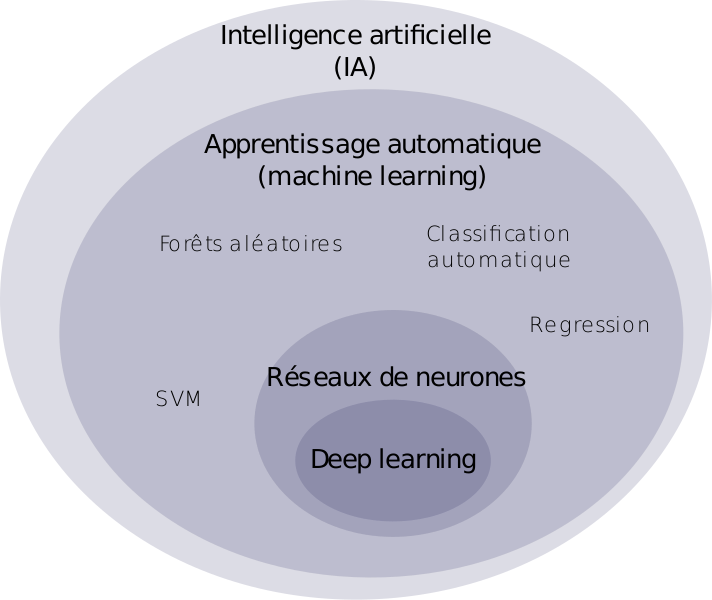
\includegraphics[width=0.7\textwidth]{Images/aitype}
            \caption{Les différents domaines de l'Intelligence Artificielle}
            \label{fig:DiffDomaineIA}
        \end{figure}

        \subsection{Shallow Learning}
            Le Machine Learning est un ensemble de techniques qui permettent à un ordinateur
            d'agir et d'apprendre comme un humain tout en s'améliorant au fur et
            à mesure et ce de manière autonome. \newline

            Le fonctionnement du machine learning se découpe en plusieurs parties,
            tout d'abord il faut définir des features, c'est-à-dire des
            propriétés mesurables individuellement, cette partie est difficile et cruciale
            car elle va déterminer l'efficacité de l'algorithme de machine learning. \newline

            Différents algorithmes vont ensuite servir à extraire les features de données
            brut en entrée avant de les envoyer à l'algorithme de machine learning, par exemple
            la reconnaissance de bords ou de forme géometriques extrait les features d'une
            image dans une IA de reconnaissance d'image. \newline

            Enfin l'algorithme de machine learning va passer au travers de 3 ensembles de données:
            \begin{itemize}
                \item un ensemble d'entraînement va permettre d'entraîner l'algorithme de manière
                supervisé, ce ensemble utilise des vecteurs d'entrée et leur sortie attendue.
                \item un ensemble de validation qui va vérifier le modèle crée à partir de l'ensemble
                d'entraînement.
                \item un ensemble de test qui permet de tester la version finale de l'algorithme.
                \newline
            \end{itemize}

            Le machine learning utilise les "réseaux de neurones", qui ont fait leurs premières
            apparition à partir de 1980, il s'agit de structures algorithmiques imitant
            le comportement des neurones dans le cerveau humain:


            \begin{figure}[H]
                \centering
                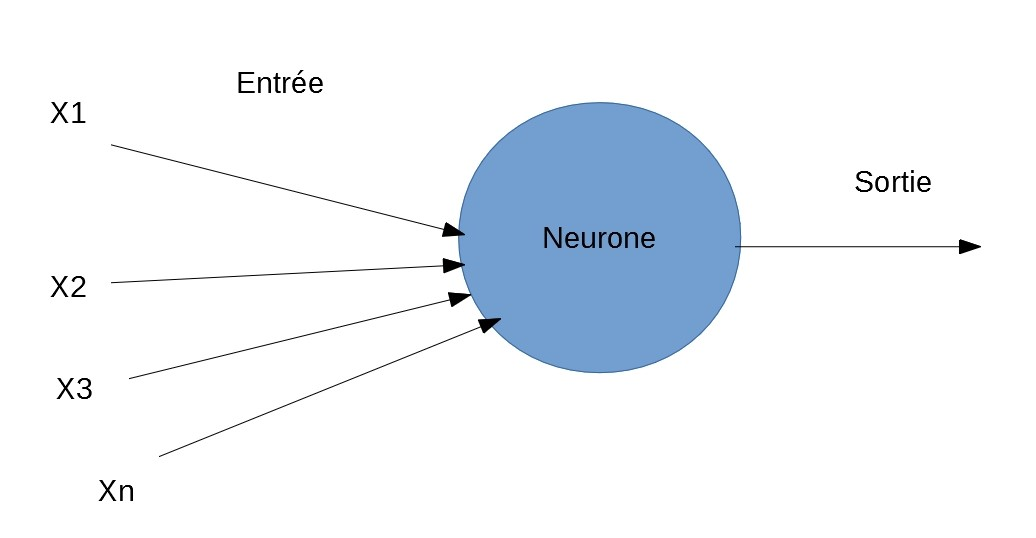
\includegraphics[width=0.6\textwidth]{Images/neuroneartificiel}
                \caption{Neurone Biologique et Neurone Artificiel}
                \label{fig:NN2Layers}
            \end{figure}

            Un neurone artificiel comme son nom l'indique imite la topologie d'un neurone biologique,
            ses entrées sont comparables aux dendrites d'un neurone tandis que sa
            sortie est l'équivalent de l'axone. \newline

            Les neurones sont répartis sur différentes couches: couche d'entrée, couche(s) cachée(s)
            et couche de sortie. Dans le cas du "shallow learning" (apprentissage superficiel,
            en opposition à l'apprentissage profond : "Deep Learning"), le réseaux de neurones
            n'est composé que d'une seule couche cachée, c'est-à-dire une seule couche entre
            la couche d'entrée et la couche de sortie:

            \begin{figure}[H]
                \centering
                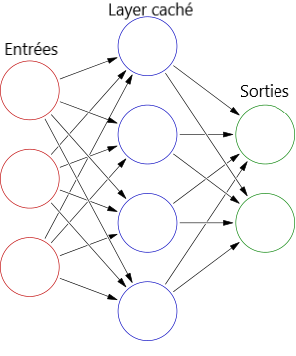
\includegraphics[width=0.4\textwidth]{Images/shallownnoverview}
                \caption{Réseau de neurones avec 2 couches cachées}
                \label{fig:NN2Layers}
            \end{figure}

            Ce type de réseaux de neurones est entrainé de manière supervisée.
            L'IA va apprendre en utilisant des exemples qui auront été décrits
            et expliqués (précision sur le degré de validité) au préalable.

            Mais dès lors qu'il y a plus d'une couche cachée,
            il n'est plus possible de l'entrainer ainsi.
            L'alternative qui répond à ce problème est l'apprentissage profond ou
            Deep Learning qui utilise des réseaux de neurones avec de multiples couches
            cachées.


        \subsection{Deep Learning}
            Le Deep Learning est une sous-catégorie du machine learning qui s'est démocratisé
            qu'à partir de 2010 et est une évolution des anciennes techniques de Machine Learning.
            La différence majeure entre ces techniques réside dans le fonctionnement du traitement des
            informations, le Shallow Learning, en contraste avec le Deep
            Learning, réside dans la nécessité de sélectionner manuellement les features
            qui doivent être identifiées par l'algorithme de machine learning:

            \begin{figure}[H]
                \centering
                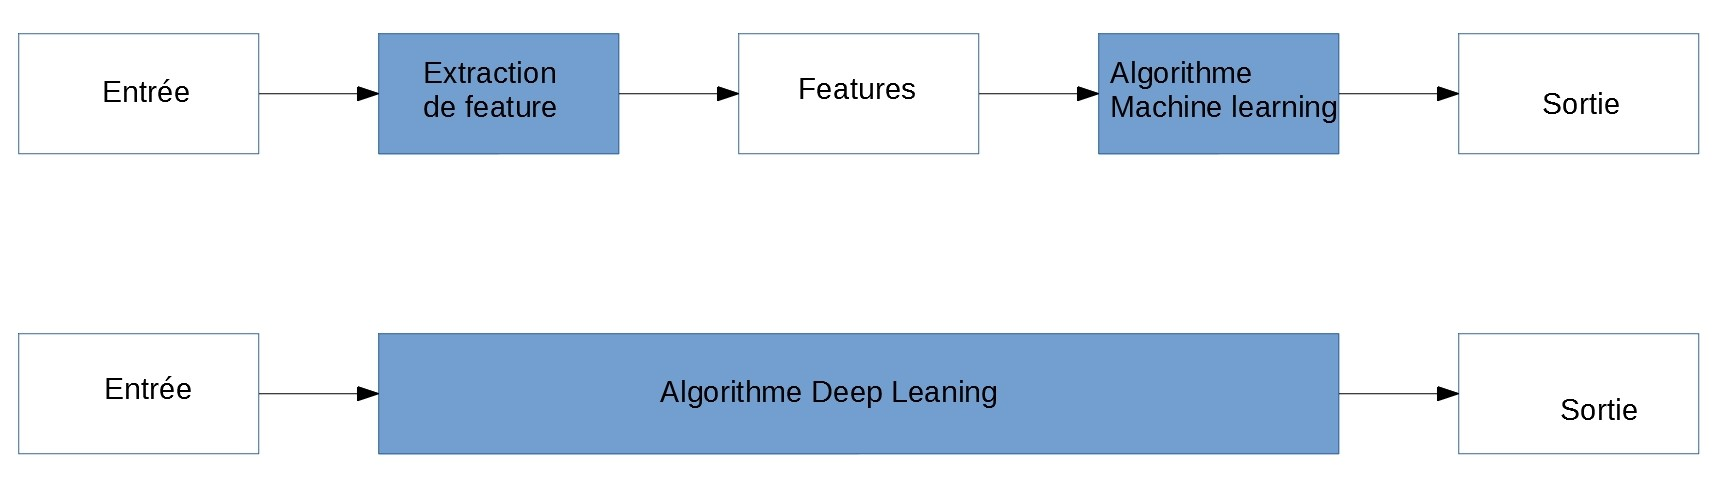
\includegraphics[width=1\textwidth]{Images/MLvsDL}
                \caption{Différences entre Shallow Learning et Deep Learning}
                \label{fig:DiffMLDL}
            \end{figure}

            Le Deep Learning contrairement au Machine Learning n'a pas besoin de sélectionner
            ou extraire manuellement les features, le modèle apprend par lui même à reconnaître
            des features, les réseaux de neurones utilisés pour le Deep Learning
            ont plus d'une couche caché de neurones d'où le nom "deep": \newline

            \begin{figure}[H]
                \centering
                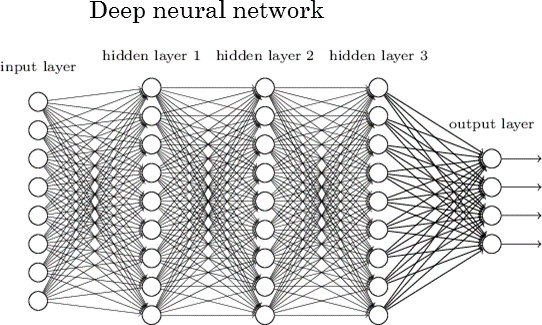
\includegraphics[width=0.7\textwidth]{Images/deepnn}
                \caption{Réseaux de neurones à 3 couches cachées}
                \label{fig:deepneuralnetwork}
            \end{figure}

            Ce qui fait la puissance du Deep Learning est sa capacité à avoir des représentations
            intermédiaires d'un niveau d'abstraction faible à un niveau d'abstraction élevé:

            \begin{figure}[H]
                \centering
                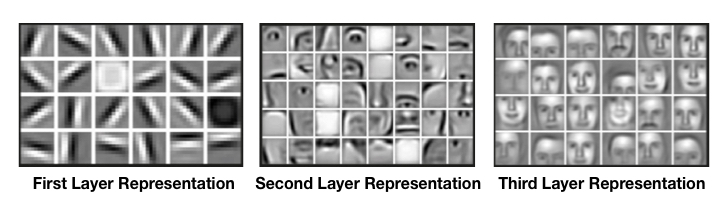
\includegraphics[width=1\textwidth]{Images/layeredrepresentation}
                \caption{Représentations intermediaires - Andrew Ng}
                \label{fig:deepnnrepresentation}
            \end{figure}

            Ces représentations permettent de ne pas avoir à définir manuellement les features.
            Dans l'exemple ci-dessus, l'algorithme extrait des features bas niveau dans la
            première représentation, puis les assemble pour former des parties des
            visages. Progressivement, l'IA obtient des représentations de features de plus en plus
            haut niveau qui finissent par former des visages entiers. \newline

\chapter{Applications de l'Intelligence Artificelle}
    Depuis ces dernières années, le Machine Learning est en essort à l'échelle mondiale.
    Une grande majorité des entreprises de nos jours cherchent à implémenter l'utilisation de l'IA
    afin de rester compétitifs sur le marché. \newline

    En effet le Machine Learning, est un concept prometteur
    et polyvalent sur la façon dont il peut se mettre en application.
    Nous nous intéresserons ici à deux domaines proposant deux perspectives différentes
    sur les apports ainsi que l'implémentation fonctionnelle de cette technologie.

    \section{Le secteur de la Finance}
        Jusqu'à il y a quelques années, la finance recrutait un nombre
        important de personnes afin de répondre aux objectifs quotidien
        que s'imposent les entreprises et institutions :\newline

        \begin{itemize}

            \item Une sécurisation forte et maintenue dans le temps : \newline
            Le milieu bancaire est certainement là où ce besoin se fait les plus ressentir.
            Des équipes entières d'inspecteurs sont formées afin d'analyser
            l'activité des comptes de chaque client
            afin de détecter des activités frauduleuses ou au moins suspectes. \newline
            Les données qui transitent entre ces établissements sont également
            enviées par bon nombre de personnes mal intentionnées,
            elles vont chercher tous les moyens possibles d'accéder à ces données. Ainsi,
            des moyens conséquents sont mis sur la maintenance, la recherche et l'évolution
            des techniques de sécurisation des données et des réseaux informatiques. \newline

            \item Une création de valeur stable et croissant : \newline
            Toute organisation dépendant de la valeur générée cherche cela. \newline

            \item Une optimisation des coûts opérationnels : \newline
            Les processus mis en place doivent avoir parmis leurs objectifs de
            rester simple et optimisés, que ce soit au niveau des coûts
            ou au niveau du temps passé. \newline

            \item Une capacité de conseil pour les clients investisseurs leur permettant 
            d'atteindre leur objectifs financier recherchés. \newline
        \end{itemize}

        Aujourd'hui l'application de l'intelligence artificielle dans le domaine de la finance 
        se situe de le conseil d'investissement, comment aider des particuliers et professionnels 
        à prendre des décisions d'investissements ? l'IA permet d'analyser une quantité 
        de données financière très importante pour voir où l'investissement semble le plus prometteur 
        ainsi que toute optimisation fiscale possible. \newline 

        \subsection*{Wealthfront}
            Wealthfront \footnote{<<Wealthfront est une société d'investissement automatique 
            et de gestion de patrimoine>> \newline Source: \url{https://en.wikipedia.org/wiki/Wealthfront} }
            a basé ses offres sur des algorithmes complexes financier pour créer des services,
            et à partir de 2016, la troisième génération de ses services utilisent la puissance 
            de l'intelligence artificielle, il s'agit d'une "augmentation" de ses services: 
            l'IA vient améliorer de manière importante des services déjà présent, de plus 
            la société Wealthfront garde des conseiller d'investissement humain 
            pour les investisseurs plus agé qui souhaitent garder un contact humain pour
            la gestion de leurs finances tandis que les conseillers automatisés par IA 
            cible une clientèle plus jeune attiré par le fait même d'utiliser de la technologie 
            pour la gestion de leur finance, le côté un peu technophile de la génération des "millenials". \newline

            Un des autres champ d'application qui a vu florir l'utilisation du machine learning: 
            la détection de fraude bancaire. En effet avant l'utilisation du machine learning 
            certaines transactions pouvait être signalées comme frauduleuses sans l'être réellement 
            ce qui occasionne d'une part une gêne pour le client et, par exemple, un manque à gagner pour 
            un site de vente puisque le client risque d'abandonner son achat. \newline

            L'objectif était donc de réduire au maximum le nombre de faux-positif dans 
            la détection de fraude, Mastercard est un exemple d'entreprise ayant mis 
            à son service la puissance de l'intelligence artificelle, Mastercard a
            acquis Brighterion en Juillet 2017, il s'agit d'une entreprise spécialisée 
            dans la création d'intelligence artificielle ce qui a permis à Mastercard de 
            mettre à profit leur expertise pour ajouter de nouveaux services 
            notamment un système de detection de fraude bien plus performant. \newline

            Le nouveau système antifraude est bien plus performant avec une réduction 
            de 50\% des faux-positifs, l'intelligence artificielle analyse en temps réel 
            les transactions financières et autres informations anonymisés
            pour trouver un pattern sortant du lot et pouvant être une fraude. 
            Une autre information importante est aussi utilisé: la géolocalisation 
            de la transaction, selon les propres mot d'Ajay Bhalla le président 
            global entreprise, risk and security: 
            \begin{quote}
                << Geographical information is highly useful because 
                not only does it give an overview of the types of transactions which are “normal” 
                for a particular area, it also reveals what patterns of fraudulent activity 
                are associated with it. Again, all of this information is aggregated in real time 
                as it happens. >>.
            \end{quote}
            \footnote{\url{https://www.forbes.com/sites/bernardmarr/2018/11/30/the-amazing-ways-how-mastercard-uses-artificial-intelligence-to-stop-fraud-and-reduce-false-declines/\#137e8f882165}}
            En effet ce type d'information permet d'identifier des zones d'opérations de gangs réalisant du blanchissement 
            d'argent et d'agir en conséquence comme par exemple augmenter les vérifications des transactions en fonction
            de la sensibilité du lieu géographique de celles-ci. \newline


    \section{Le secteur de la médecine}
        l'intelligence artificielle comme dans la majorité des domaines où elle est applicable est utilisée
        pour répondre à plusieurs besoin:
        \begin{itemize}
            \item Gestion de la médication: une intelligence artificelle mêlant capacité conversationnelle,
            reconnaissance faciale (pour analyser l'état du patient) et analyse de donnée de santé. \newline
            \item Rechercher assistée par Intelligence Artificielle: les algorithmes de machine learning peuvent
            être beaucoup plus performant que des algorithmes standard et plus flexible ce qui permet 
            de faire avancer la recherche plus rapidement. \newline 
            \item Analyse de systèmes de santé: une IA permet d'analyser une quantité conséquente de données 
            pour trouver d'éventuelles erreurs notamment de la mise en place de traitement par exemple.
        \end{itemize}

        \subsection*{AtomNet}
            AtomNet est une technologie développé par la société AtomWise,
            il s'agit d'une intelligence artificelle utilisant un réseau de neurone convolutif
            \footnote{Un réseau de neurone convolutif est un réseau ou les neurones sont en plusieurs 
            couches, chaque couche ne communique qu'avec la suivante, très couramment utilisé dans le
            traitement d'image et le traitement du langage naturel.
            Source: \url{https://fr.wikipedia.org/wiki/R\%C3\%A9seau_neuronal_convolutif}}
            utilisé pour la recherche de nouveaux traitements.
           \begin{quote}
            << la plus grosse difficulté aujourd'hui dans la recherche de traitement médicaux 
            est d'identifier un traitement candidat qui est à la fois efficace et sûr, un problème 
            que rencontre les chercheurs dans des milliers d'institution. >> 
            \footnote{Source: \url{https://www.atomwise.com/our-technology/}}
            \end{quote}
            La solution que propose AtomWise avec son produit AtomNet est d'utiliser la puissance 
            des réseaux de neurones convolutif pour accelerer la recherche, un de point de congestion
            très un important dans celle-ci est le repliement de proteine ou comment une protéine 
            prend sa forme en trois dimension qui lui permet de devenir fonctionnel, ce type de connaissance 
            est essentiel pour permettre le développement de nouveaux médicaments or les 
            algorithme traditionnel sont beaucoup moins performant pour identifier des patterns
            de repliement comparé à des réseaux de neurones qui eux peuvent analyser les repliement 
            de protéines et tester des composé chimiques beaucoup plus rapidement que ce dont 
            l'humain est capable. \newline 

            l'intelligence artificelle fonctionne avec des entrée visuelles en utilisant en lieu et place 
            des couleurs des type d'atome, cela permet de faire un assemblage créant des molécules et 
            protéines, AtomNet apprend ainsi comment se font les liaisons entre molécules à partir de 
            données d'entrainement. \newline
            \newpage

        \subsection*{Babylon}
            Babylon est un service en ligne de consultation basé sur l'intelligence artificelle, 
            avec un système de conversation "chat":
            \begin{quote}
                << elle peut comprendre et reconnaitre la manière 
                unique que les humains utilisent pour exprimer leurs symptômes. en utilisant ces 
                connaissances en combinaison avec l'historique médical du patient et les symptômes
                actuels, elle peut donner des informations sur les possible conditions médical 
                que subis l'utilisateur et les traitements commun. >>
            \end{quote}
            les techniques utilisées pour le fonctionnement de Babylon sont toutes 
            augmentées avec l'utilisation du machine learning: \newline
            \begin{itemize}
                \item Graphe de connaissance: un type de base de connaissance
                    \footnote{
                        << Une base de connaissance regroupe des connaissances spécifiques à un 
                        domaine spécialisé donné, sous une forme exploitable par un ordinateur. 
                        Elle peut contenir des règles (dans ce cas, on parle de base de règles), 
                        des faits ou d'autres représentations >> \newline 
                        source: \url{https://fr.wikipedia.org/wiki/Base_de_connaissance}
                    }
                    qui liste une grande quantité d'informations médicales transformées 
                    pour pouvoir être utilisées par une intelligence artificelle, 
                    ce graphe est utilisé par tout les autres systèmes intelligent 
                    de Babylon, il est aussi en connexion avec le graphe utilisateur 
                    qui lui stocke des données de cas particuliers,
                    l'objectif est d'avoir le plus d'information concises 
                    pour assister le moteur d'inférence. 
                    Le machine learning est utilisé pour transformer et ajouter de nouveaux articles 
                    de médecine et autres connaissances dans le graphe.
                    \newline

                \item Traitement automatique du langage naturel: 
                Les autres système de Babylon reçoivent en entrée des données qui ont déjà 
                été pre-traité c'est le rôle de cette partie de comprendre l'utilisateur 
                de manière conversationnelle et le plus naturellement possible car
                beaucoup de personnes sont toujours plus à l'aise en face à face 
                avec un humain qu'avec une machine. Cette partie décompose 
                le langage humain parlé et écrit pour y trouver un sens notamment avec l'aide 
                du graphe de connaissances. Le machine learning est utilisé pour accélérer exponentiellement 
                la vitesse de recherche et établir des liens entre des symptômes et conditions 
                qui n'existaient pas avant.
                \newline

                \item Moteur d'inférence: 
                << un logiciel correspondant à un algorithme de simulation des raisonnements déductifs >>
                \footnote{\url{https://fr.wikipedia.org/wiki/Moteur_d\%27inf\%C3\%A9rence}}
                C'est la partie centrale à l'intelligence artificelle de babylon, ce moteur 
                prend un ensemble de raisonnement simple pour établir diagnostique médical.
                \newline
            \end{itemize} 
            \newpage


    \section{Le secteur industriel}
        Le secteur industriel a un rapport différent avec l'intelligence artificielle car elle est arrivée 
        bien plus tard que pour les autres secteurs comme le marketing, la finance et la médecine.
        Une des spécificités de l'industrie manufacturière est la variété de ses composantes: 
        aucune chaîne de montage n'est pareil entre deux industriels qu'il produisent des bien 
        dans le même domaine ou pas mais un des autres avantages est la présence d'une forte quantité 
        d'informations avec les sondes et capteurs présents sur les chaînes de montage automatisées 
        (qui sont omniprésente surtout dans le domaine automobile et les produit de consommation électroniques), 
        mais ces informations ne sont pas forcément traitable en tant que tel et doivent être, pre-traitées
        avant d'être utilisée par une intelligence artificelle qu'elle utilise l'entrainement 
        supervisé ou l'entrainement non-supervisé. \newline

        l'utilisation de l'intelligence artificelle dans l'industrie a vu apparaître 
        l'industrie "4.0":

        \begin{figure}[H]
            \centering
            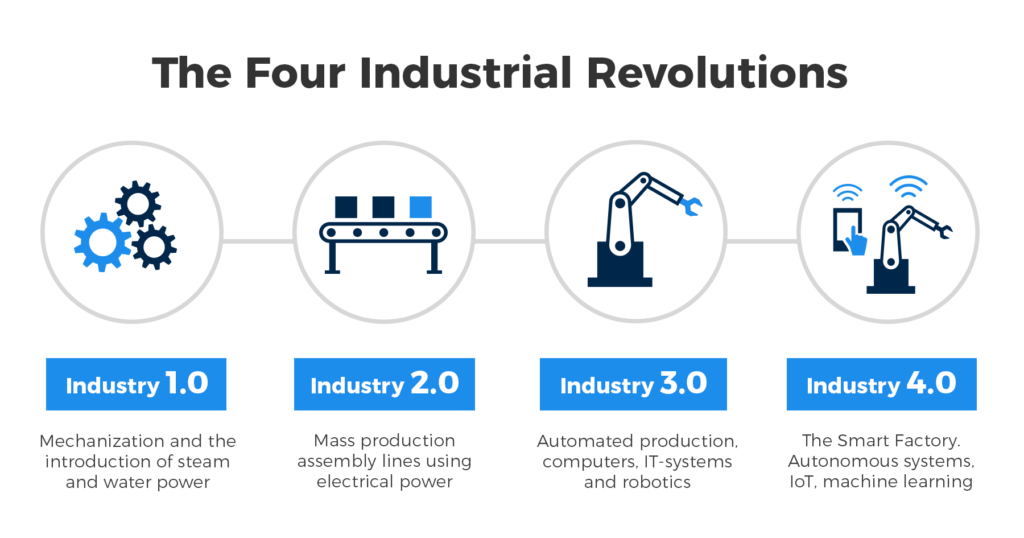
\includegraphics[width=0.8\textwidth]{Images/industryfour}
            \caption{Les quatres révolutions de l'industrie - spectralengines.com}
            \label{fig:fourindustrialrevolutions}
        \end{figure}

        Aujourd'hui l'intelligence artificelle dans l'industrie est principalement utilisée pour:
        \begin{itemize}
            \item Réduire les coûts de la main d'oeuvre grâce à la majorité des points suivants. \newline

            \item Réduire les produits défectueux ce qui est rendu possible en analysant les données
            en temps réel de la chaîne de fabrication pour toute information qui sortirait de l'ordinaire 
            telle que la différence de poids entre les pièces qui serait en dehors de la précision déterminé
            lors de design de celles-ci, ou même les dimensions avec des outils d'analyse optiques qui 
            sont capable de déterminer des erreurs de précision des machines-outils. \newline

            \item Raccourcir la durée des maintenance non-planifiées: une des grandes sources de coût sont les 
            maintenances non prévues de machine outils ou d'autres équipement sur la chaîne de production, ces
            maintenances entrainement un arrêt de la ligne concernée jusqu'a rétablissement à un état 
            opérationnel de l'équipement, une des applications de l'intelligence artificelle est la 
            prévision des pannes et des équipement qui doivent passer en maintenance en utilisant les données
            des machines pour voir une évolution dans les performances et/ou la précision.
            Un algorithme de machine learning correctement entrainé sera capable de detecter les signes 
            d'un équipement qui fatigue ou un problème de fonctionnement et ainsi manager le reste 
            de la ligne de production pour permettre la mise en maintenance de l'équipement en ayant 
            l'impact le plus minime possible sur le reste de la production. \newline 

            \item Améliorer les phases de transitions entre les différentes parties d'une 
            chaîne de production: transporter des pieces entre les différente chaque parties 
            de la chaîne est un point d'optimisation important, aujourd'hui beaucoup d'usines
            utilisent des robot transporteur entre chaque partie de la production d'un produit
            mais il est encore possible d'optimiser la coordination entre les robots pour réduire
            durée transitoire. \newline 

            \item Augmenter la vitesse de production: Le machine learning permet d'identifier les point 
            de congestion dans un processus industriel et de mettre au point des solutions pour les éradiquer 
            ou minimiser ce qui à pour résultat d'augmenter la vitesse de production, ce qui est bien 
            plus économique que d'agrandir les chaînes de production. \newline 

            \item Design de produit: l'intelligence artificelle peut être utilisé pour optimiser les propriétés 
            physique des produits réalisés ou leurs propriétés de fonctionnement, en ce basant sur une
            version simulé du produit les coût de conception étaient déjà grandement réduits 
            (pas besoin de fabriquer le produit pour faire des tests) mais avec l'avènement de 
            l'intelligence artificelle ces derniers sont encore plus faibles grâce à des performances
            encore plus fortes qui minimisent les cycles de développements.
            \newline
        \end{itemize}

        \subsection*{Siemens}
            Siemens \footnote{<< Siemens est un groupe 
            international d’origine allemande spécialisé dans les secteurs de l'énergie, 
            de la santé, de l'industrie et du bâtiment. 
            Il a été fondé en 1847 par Werner von Siemens. 
            Le groupe, dont le siège est à Munich, est le premier employeur privé d'Allemagne, 
            et la plus grande société d'ingénierie (en termes d'effectifs) en Europe >> 
            Source: \url{https://fr.wikipedia.org/wiki/Siemens}}
            utilise le deep learning dans les différents process de ses usines d'acier,
            et en Mars 2016 lance Mindsphere: 
            << Mindsphere a été conçu en tant qu'éco-système ouvert que les entreprises industrielles
            peuvent utiliser comme base pour leur propres services digitaux, comme par exemple pour 
            le domaine de la maintenance préventive, la gestion des données de consommation et 
            l'optimisation de ressources. les fabricant de machine et constructeurs d'usines
            peuvent utiliser la plateforme pour surveiller des flottes de machine proposant des
            services partout dans le monde, réduire leur temp d'indisponibilitée et 
            conséquemment offrir de nouveaux business models. >> 
            \footnote{Traduction extraite de: \url{https://www.siemens.com/press/en/pressrelease/?press=/en/pressrelease/2016/digitalfactory/pr2016030171dfen.htm}}
            \newline

            Siemens a aussi commencé en 2017 une recherche pour réaliser un système d'analyse 
            de donnée en temps réel utilisant un casque de réalité virtuelle pour visionner 
            un modèle 3D d'une vrai turbine à gaz (le type de turbine utilisé dans les 
            centrales éléctriques, centrales nucléaires), une intelligence artificelle reçois les 
            informations de centaines de capteurs sur la turbine réelle et les interpretes
            pour les transposer sur la version "digitales", cela permet d'effectuer
            des vérifications sans interrompre le fonctionnement de la machine 
            et même trouver de possible problèmes ou signes de fatigues mécanique. \newline
            Ce type de produit novateur et inédit sur le marché associé à 
            un stockage des données dans le cloud permettra une maintenance 
            des machines complexes à distance où que ce soit dans le monde. \newline 

            \begin{figure}[H]
                \centering
                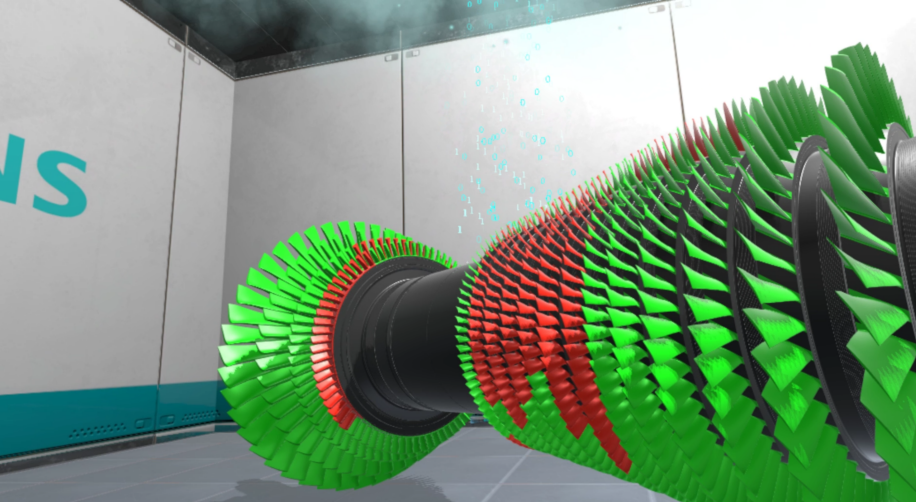
\includegraphics[width=0.5\textwidth]{Images/turbine}
                \caption{simulation en réalité virtuelle d'une turbine à gaz - siemens.com}
                \label{fig:gasturbine}
            \end{figure}


            Click2Make est encore une autre technologie en développement chez Siemens 
            qui pourrait changer radicalement le paysage des fabricant industriels
            en transformant des grandes ligne de fabrication en cellule de production 
            et proposant du "production-as-a-service": \newline
            \begin{itemize}
                \item Un client fait une demande pour manufacturer un produit
                \item Le système effectue une offre.
                \item Chaque cellule de production contient une liste de ses capacité machines et 
                humaines qui l'envoie au système.
                \item Le système reunis les ressources nécéssaire pour la fabrication de la manière
                la plus optimisé possible et avec le coût le plus bas. \newline
            \end{itemize}


            De plus Click2Make semble convenir particulierement à l'impression 3D qui est 
            en croissance constante depuis plusieurs années et permet même aujourd'hui 
            d'imprimer des piece avec des matériaux et alliage complexes tel que le titane avec 
            les étriers de freins bugatti réalisés via ce procédé. 
            \newpage


        \subsection*{Fanuc}
            Fanuc est une entreprise japonaise leader dans les robots industriels et les machines CNC 
            \footnote{Computer Numerical Control, Commande Numérique par Ordinateur en Français}
            valué à plus de 40 milliards de dollars, cette entreprise a aussi des usines de "fabrication dans le noir"
            c'est à dire des usines completement autonomes qui ne nécéssitent pas d'intervention humaine dans les 
            lignes de production, les matières premières sont fournies en entrée et les produit sont 
            disponible en sortie. Ce type d'usine permet de consommer beaucoup moins d'éléctricité car en l'absence 
            d'être humain des les batiments il n'y pas besoin de lumière, climatisation ou chauffage et permet
            aussi de continuer à produire la nuit ou le weekend. \newline

            Cette entreprise a développé un robot capable d'apprendre une tâche lui même au bout 
            d'une nuit d'entrainement en utilisant le reinforced deep learning. Les robot industriels 
            ont été (et le sont toujours pour certains langages) programmés avec des langages fait pour les PLC 
            ou Programmable Logic Controller tel que GRAFCET, LADDER et consorts. 
            développer ces programmes nécéssite un expert dans le domaine et est donc un coût, 
            avec l'avènement de l'intelligence artificelle ce coût viendra à disparaître tout 
            en rendant ces robots bien plus flexibles au changement qu'avec un programme fixe. \newline

            Le robot utilise un enrengistrement vidéo de lui même pour alimenter le réseau de neurones,
            il répète l'action voulu jusqu'a se rapprocher de la précision demandé,
            de plus l'architecture de la technologie permet de combiner plusieurs machine pour combiner 
            leur entrainement et accélérer l'apprentissage de la tâche, on pourrais imagine qu'une tâche 
            nécéssitant 8h d'entrainement avec une seule machine pourrait en prendre que deux 
            avec la combinaisons de quatres machines, les robots avec des tâches simples et répétitives 
            tel que les robot de mise sous emballage sont les cibles privilégiés pour tester et 
            améliorer cette technologie. \newline 

            Contrairement à la programmation "standard" le robot acquiere un savoir 
            plus général tel que comment manipuler des catégorie d'objet qui ont 
            des caractéristiques en commun, ce nouveau type de connaissances alliées au cloud 
            et à l'internet des objects va redéfinir l'industrie, mais cela reste un domaine 
            de la recherche et du développement de Fanuc car appliquer le deep learning 
            n'est pas une chose aisée, les applications se rapproche des performances qui se rapprochent 
            de celle que celle d'une intelligence artificelle à apprentissage générique (une 
            IA qui n'est pas isolée à un seul domaine d'apprentissage tel que la reconnaissance d'image)
            et les chercheurs avancent encore à taton, malgré les résultats probants 
            l'industrie ne va pas encore voir se démocratiser les robot "augmenté" par l'IA. \newline
            \newpage






